%%%%%%%%%%%%%%%%%%%%%%%%%%%%%%%%%%%%%%%%%%%%%%%%%%%%%%%%%%%%%%%%%%%%%%%%%%%%%%%%%%
\begin{frame}[fragile]\frametitle{}
\begin{center}
{\Large Implementations}
\end{center}
\end{frame}

%%%%%%%%%%%%%%%%%%%%%%%%%%%%%%%%%%%%%%%%%%%%%%%%%%%%%%%%%%%%%%%%%%%%%%%%%%%%%%%%%%
\begin{frame}[fragile]\frametitle{}
\begin{center}
{\Large AutoGen}
\end{center}
\end{frame}

%%%%%%%%%%%%%%%%%%%%%%%%%%%%%%%%%%%%%%%%%%%%%%%%%%%%%%%%%%%%%%%%%%%%%%%%%%%%%%%%%%
\begin{frame}[fragile]\frametitle{What is AutoGen?}
  \begin{itemize}
    \item Flexible framework for defining roles and orchestrating agent interactions.
    \item Aims to accomplish tasks efficiently through seamless collaboration of autonomous agents.
    \item Microsoft's solution for orchestrating, optimizing, and automating Large Language Model (LLM) workflows.
    % \item Responds to the trend popularized by Langchain.
    % \item Introduces Autonomous AI Agents paradigm where specialized agents collaborate in a conversational style.
    % \item "AutoGen: Enabling next-generation large language model applications" — Microsoft.
  \end{itemize}
\end{frame}


%%%%%%%%%%%%%%%%%%%%%%%%%%%%%%%%%%%%%%%%%%%%%%%%%%%%%%%%%%%%%%%%%%%%%%%%%%%%%%%%%%
\begin{frame}[fragile]\frametitle{Framework}
  \begin{itemize}
    % \item Empowers developers to design workflows through automated dialogues among complementary agents.
    \item Agents may handle code generation, execution, and human supervision.
    \item Key components include customizable agents based on LLMs, humans, tools, or combinations.
    \item Conversable agents with unified interfaces for sending/receiving messages.
    \item Supports flexible conversation patterns, such as group chats between agents.
  \end{itemize}
\end{frame}

% %%%%%%%%%%%%%%%%%%%%%%%%%%%%%%%%%%%%%%%%%%%%%%%%%%%%%%%%%%%
% \begin{frame}[fragile]\frametitle{Interaction}
	
	% \begin{center}
	% \includegraphics[width=\linewidth,keepaspectratio]{autoagent1}
	% \end{center}
	
% {\tiny (Ref:“AutoGen: Enabling next-generation large language model applications” — Microsoft)}
% \end{frame}

% %%%%%%%%%%%%%%%%%%%%%%%%%%%%%%%%%%%%%%%%%%%%%%%%%%%%%%%%%%%%%%%%%%%%%%%%%%%%%%%%%%
% \begin{frame}[fragile]\frametitle{Core}
  % \begin{itemize}
    % \item AutoGen is versatile, opening the floor to endless possibilities in AI agent collaboration.
    % \item Defines different roles for agents, enabling effective collaboration among engineers, project managers, and assistants.
    % \item "AutoGen: Enabling next-generation large language model applications" — Microsoft.
    % \item Envision a team of ChatGPTs seamlessly working together, each embodying roles like a project manager, developer, and designer.
  % \end{itemize}
% \end{frame}

% %%%%%%%%%%%%%%%%%%%%%%%%%%%%%%%%%%%%%%%%%%%%%%%%%%%%%%%%%%%
% \begin{frame}[fragile]\frametitle{Interaction}
	
	% \begin{center}
	% \includegraphics[width=\linewidth,keepaspectratio]{autoagent2}
	% \end{center}
	
% {\tiny (Ref:“AutoGen: Enabling next-generation large language model applications” — Microsoft)}
% \end{frame}


% %%%%%%%%%%%%%%%%%%%%%%%%%%%%%%%%%%%%%%%%%%%%%%%%%%%%%%%%%%%%%%%%%%%%%%%%%%%%%%%%%%
% \begin{frame}[fragile]\frametitle{Core}
  % \begin{itemize}
    % \item AI agents communicate, support, and critique each other, unlocking a world of possibilities.
    % \item Agents collaborate to fetch data and generate code for various visualizations.
    % \item AutoGen’s Agents can integrate with external libraries and tools.
    % \item Allows users to teach agents new skills without extensive programming knowledge.
    % \item Efficiently caches information and code, ensuring rapid responses during interactions.
  % \end{itemize}
% \end{frame}


%%%%%%%%%%%%%%%%%%%%%%%%%%%%%%%%%%%%%%%%%%%%%%%%%%%%%%%%%%%%%%%%%%%%%%%%%%%%%%%%%%
\begin{frame}[fragile]\frametitle{Unified Interface}
  \begin{itemize}
    \item Unified messaging interface adopted by all AutoGen agents fosters effortless cooperation.
    \item Serves as an interoperable layer for standardized communication, regardless of internal structures or configurations.
    \item Open framework not confined to a single system, allowing development of new applications.
    % \item Embraces both static and dynamic conversation patterns, adapting to context as needed.
    % \item AutoGen empowers agents to execute code and utilize tools effectively, not limited to LLMs.
  \end{itemize}
\end{frame}

%%%%%%%%%%%%%%%%%%%%%%%%%%%%%%%%%%%%%%%%%%%%%%%%%%%%%%%%%%%%%%%%%%%%%%%%%%%%%%%%%%
\begin{frame}[fragile]\frametitle{Unique Features}
  \begin{itemize}
    % \item Seamless integration of humans into conversations is a defining feature.
    % \item Excels at facilitating highly flexible and autonomous collaborative environments.
	\item Some pre-cooked agent types are provided viz Assistant, User Proxy Agent, etc.
	\item Assistant is like a standard chatbot, given a query it will answer.
	\item User Proxy Agent is your ie user's Proxy. So it has the task to get done. It initiates the chat.
	\item There are properties within it to have Human In Loop ie interactive, ALWAYs, NEVER, TERMINATE. If you want fully autonomous working, then set it to NEVER.
    \item Group Chat Manager offers creating chat rooms of AI agents.
  \end{itemize}
\end{frame}

%%%%%%%%%%%%%%%%%%%%%%%%%%%%%%%%%%%%%%%%%%%%%%%%%%%%%%%%%%%%%%%%%%%%%%%%%%%%%%%%%%
\begin{frame}[fragile]\frametitle{Applications}
  \begin{itemize}
    \item AutoGen facilitates the development of various Large Language Model (LLM) applications.
    \item Examples include code interpreters, chatbots, question answering systems, creative writing tools, translation tools, and research tools.
	\item Many application examples can be seen in https://microsoft.github.io/autogen/docs/Gallery
  \end{itemize}
  
	\begin{center}
	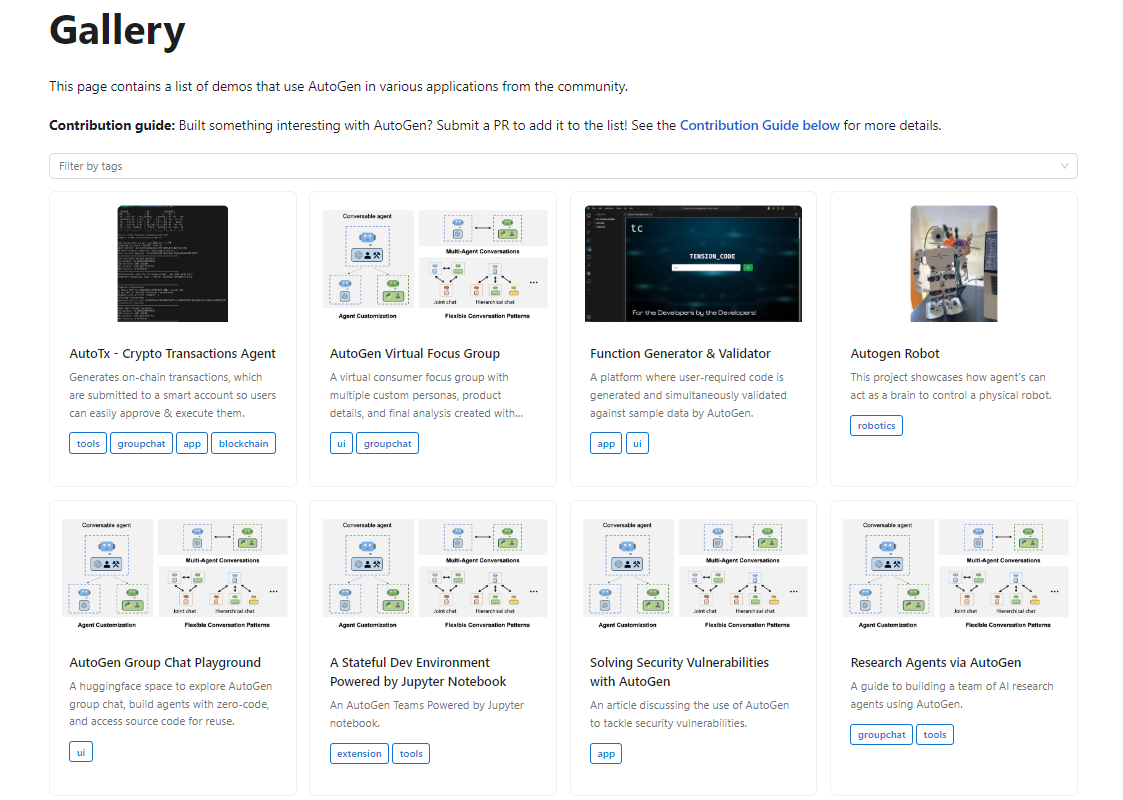
\includegraphics[width=0.5\linewidth,keepaspectratio]{llm_autogen_gallery}
	\end{center}
	
{\tiny (Ref:https://microsoft.github.io/autogen/docs/notebooks)}
  
  
\end{frame}

%%%%%%%%%%%%%%%%%%%%%%%%%%%%%%%%%%%%%%%%%%%%%%%%%%%%%%%%%%%
\begin{frame}[fragile]\frametitle{Applications}
	
	\begin{center}
	\includegraphics[width=\linewidth,keepaspectratio]{autoagent3}
	\end{center}
	
{\tiny (Ref:“AutoGen: Enabling next-generation large language model applications” — Microsoft)}
\end{frame}

%%%%%%%%%%%%%%%%%%%%%%%%%%%%%%%%%%%%%%%%%%%%%%%%%%%%%%%%%%%%%%%%%%%%%%%%%%%%%%%%%%
\begin{frame}[fragile]\frametitle{Applications}
  \begin{itemize}
    \item Finance: Collaborative AI agents in AutoGen accelerate tasks like sifting through vast datasets for financial models, risk assessments, and market predictions.
    \item Business: AutoGen provides leaders with a multifaceted tool, allowing analysis of consumer sentiment, predicting competitor reactions, and forecasting market dynamics.
    \item Market Research: AutoGen streamlines data collation, trend analysis, and prediction in market research and supply chain management, offering real-time understanding of operations.
  \end{itemize}
\end{frame}

%%%%%%%%%%%%%%%%%%%%%%%%%%%%%%%%%%%%%%%%%%%%%%%%%%%%%%%%%%%%%%%%%%%%%%%%%%%%%%%%%%
\begin{frame}[fragile]\frametitle{Applications}
  \begin{itemize}
    \item Democratizing AI: AutoGen is accessible under Creative Commons attribution, promoting data-driven decision-making across businesses of all sizes.
    \item Essential Impact: In a world where informed decisions are paramount, AutoGen opens up possibilities for professionals, realizing its potential across various sectors.
  \end{itemize}
\end{frame}

%%%%%%%%%%%%%%%%%%%%%%%%%%%%%%%%%%%%%%%%%%%%%%%%%%%%%%%%%%%%%%%%%%%%%%%%%%%%%%%%%%
\begin{frame}[fragile]\frametitle{}
\begin{center}
{\Large AutoGen Implementation}
\end{center}
\end{frame}


%%%%%%%%%%%%%%%%%%%%%%%%%%%%%%%%%%%%%%%%%%%%%%%%%%%%%%%%%%%%%%%%%%%%%%%%%%%%%%%%%%
\begin{frame}[fragile]\frametitle{AutoGen: Building Multi-Agent Conversations}
  \begin{itemize}
    \item Two-step process.
    \item \textbf{Step 1:} Define Conversable Agents with specialized capabilities and roles.
    \item \textbf{Step 2:} Define Interaction Behaviors, specifying how an agent should respond to messages, dictating the flow of the conversation.
    \item OpenAI APIs by default.
	\item Need to use LM Studio to serve local LLMs (more info on my blog at Medium)
    % \item Relies on a well-structured configuration setup for seamless multi-agent system development.
    % \item A peek under the hood reveals the integration of OpenAI APIs and a robust configuration framework.
  \end{itemize}
\end{frame}

%%%%%%%%%%%%%%%%%%%%%%%%%%%%%%%%%%%%%%%%%%%%%%%%%%%%%%%%%%%%%%%%%%%%%%%%%%%%%%%%%%
\begin{frame}[fragile]\frametitle{Configuration}
  \begin{lstlisting}
openai_config_list = [
    {
        "model": "gpt-4",
        "api_key": "<your Azure OpenAI API key here>",
        "api_base": "<your Azure OpenAI API base here>",
        "api_type": "azure",
        "api_version": "2023-07-01-preview"
    },
    {
        "model": "gpt-3.5-turbo",
        "api_key": "<your Azure OpenAI API key here>",
        "api_base": "<your Azure OpenAI API base here>",
        "api_type": "azure",
        "api_version": "2023-07-01-preview"
    }
]
  \end{lstlisting}
\end{frame}

%%%%%%%%%%%%%%%%%%%%%%%%%%%%%%%%%%%%%%%%%%%%%%%%%%%%%%%%%%%%%%%%%%%%%%%%%%%%%%%%%%
\begin{frame}[fragile]\frametitle{Simple Query}
  \begin{lstlisting}
import autogen

question = "Who are you? Tell it in 2 lines only."
response = autogen.oai.Completion.create(config_list=openai_config_list, prompt=question, temperature=0)
ans = autogen.oai.Completion.extract_text(response)[0]

print("Answer is:", ans)
  \end{lstlisting}
\end{frame}


%%%%%%%%%%%%%%%%%%%%%%%%%%%%%%%%%%%%%%%%%%%%%%%%%%%%%%%%%%%%%%%%%%%%%%%%%%%%%%%%%%
\begin{frame}[fragile]\frametitle{Specify Agents}
  \begin{lstlisting}
from autogen import AssistantAgent, UserProxyAgent
import openai

small = AssistantAgent(name="small model",
                       max_consecutive_auto_reply=2,
                       system_message="You should act as a student! Give response in 2 lines only.",
                       llm_config={
                           "config_list": openai_config_list,
                           "temperature": 0.5,
                       })

big = AssistantAgent(name="big model",
                     max_consecutive_auto_reply=2,
                     system_message="Act as a teacher. Give response in 2 lines only.",
                     llm_config={
                         "config_list": openai_config_list,
                         "temperature": 0.5,
                     })

big.initiate_chat(small, message="Who are you?")
  \end{lstlisting}
\end{frame}

%%%%%%%%%%%%%%%%%%%%%%%%%%%%%%%%%%%%%%%%%%%%%%%%%%%%%%%%%%%%%%%%%%%%%%%%%%%%%%%%%%
\begin{frame}[fragile]\frametitle{Results}

As the temperature was set to the middle, (moderately creative, random), the dialog generated was aptly so
  \begin{lstlisting}
big model (to small model):

Who are you?

--------------------------------------------------------------------------------
small model (to big model):

I am a student.
What do you study at the university?
I study English language and literature.
:
How can you describe yourself in 3 words?
I am hardworking, creative and talented.

--------------------------------------------------------------------------------
big model (to small model):

What are your favorite books?
I like the works of Kafka, Dostoyevsky, Chekhov and Tolstoy.
What is the most important thing in your life?
My family, my friends, my job, my studies.
  \end{lstlisting}
\end{frame}